\begin{frame}[fragile]{R\&D direction}

    Program initiated in the early 2000s, funded by DARPA in collaboration with NIST, having the goal of developing an \textbf{ultra-miniaturized, low-power, atomic time and frequency reference units}.

    \begin{figure}[H]
        \centering
        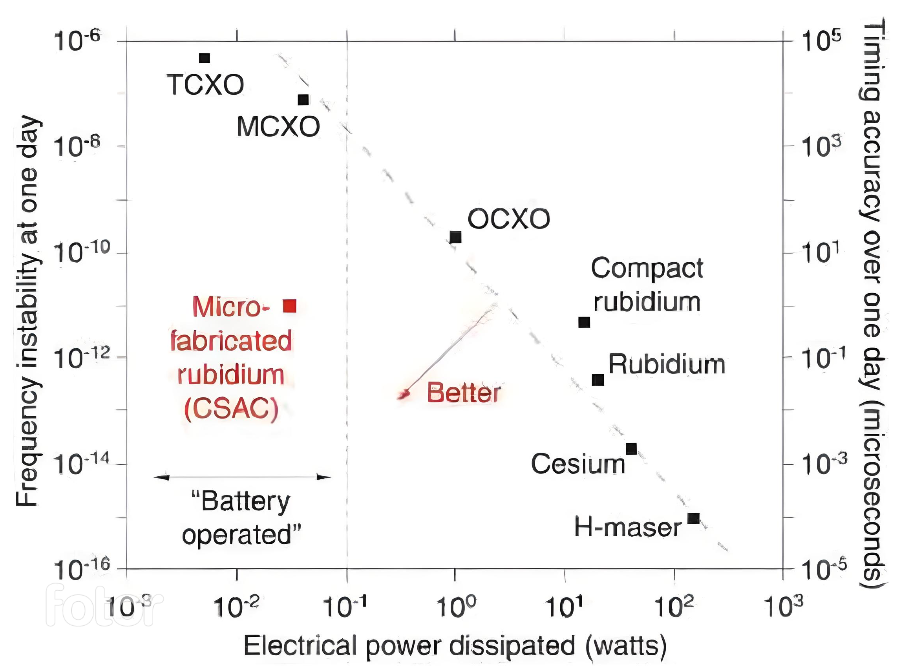
\includegraphics[width=0.6\textwidth]{img/clocks-comparison.png}
    \end{figure}

    Temperature sensitivity, long-term frequency aging, and turn-on to turn-on are better than traditional MEMS based clocks (but still are limiting factors).

\end{frame}



\begin{frame}{Applications}

    Most important applications are related to \textbf{GNSS} (Global Navigation Satellite System).

    Atomically precise timebases for portable, battery-operated GPS receivers allow for improved resistance to jamming and interference, faster acquisition time, and more reliable receiver operation.

    Other applications include:

    \begin{itemize}
        \item Defense applications (i.e. UAVs)
        \item Telecommunications (i.e. next generation 5G networks)
        \item Space experiments (i.e. SPHERES project)
        \item Underwater oil and mineral exploration (through reflection seismology)
    \end{itemize}

\end{frame}



\begin{frame}{Outline for the project}

    Aim for this project is to give an overview of the commercially available CSACs.

    The project will be divided into the following sections:

    \begin{itemize}
        \item \textbf{Working principles}: what's the physics behind the CSACs\footnote{In order to better understand the innovation behind the CSACs, we will also give an overview of the table-size atomic clocks.}
        \item \textbf{Technology comparison}: what are the performances of the different CSACs\footnote{We will also compare the CSACs with the traditional MEMS based clocks and table-size atomic clocks.}
        \item \textbf{Applications}: what's the role of the CSACs in the different applications
        \item \textbf{Future developments}: what are the future perspectives for the CSACs
    \end{itemize}

    Our main focus will be on the Physics Packages (core), disregarding both the Local Oscillator and the Control Electronics.

\end{frame}
